% !TEX root = ../main.tex

\chapter{Experimental setup}\label{chap:cms}

Today, the Higgs boson and  particles of the second and third generation do not appear very frequently in the universe anymore. When the temperature dropped below their rest masses, they left thermal equilibrium and decayed more or less instantly into more stable particles. 
They are created in high-energy processes such as the interaction of cosmic rays with the atmosphere making it difficult or impossible to study their properties in nature.
Elementary particles have to be produced artificially to study their properties in a reproducible and unbiased environment. To reach energy densities comparable to the first seconds of the universe,
physicists build particle colliders that accelerate charged, stable particles or nuclei to highest energies and scatter them at fixed targets or collide them with an oppositely accelerated beam of particles transforming such kinetic energy eventually into mass.
Sophisticated detector systems, constructed to detect and reconstruct particles produced in the collisions, are built around the interaction point. Thus, the signature of the decay of an unstable particle
eventually created in a particle collision, is recorded.
In this thesis, an analysis using a data set of proton-proton collisions collected at the Large Hadron Collider (LHC) from Run 2 corresponding to an
integrated luminosity of $\text{35.9\,fb}^\text{-1}$ is performed. The data was recorded by the CMS Detector during the year 2016. 

\section{The Large Hadron Collider}\label{sec:LHC}

The LHC at CERN is a particle accelerator and storage ring that is capable of accelerating protons to a maximum energy of currently 6.5\,{TeV} and bringing them into collision at so-called interaction points. 
The ring has a circumference of 26.7\,km and is operated in the old LEP tunnel near Geneva. 
It is currently the largest and most powerful particle accelerator in the world. 
A sketch showing the full LHC complex including relevant pre-acceleration steps is given in \figreft{CMS:LHC_overview}. 
The LHC uses superconducting radio-frequency cavities (RF cavities) operating at a frequency of 400.8\,MHz to accelerate proton bunches in opposite directions. Superconducting dipole magnets with field strengths of up to 8\,{T} force the bunches on a circular orbit \cite{lhc_machine}.
The LHC as storage ring keeps the beams in circulation with a lifetime of \sim 12\,h. During that time proton bunches collide every 25\,ns at the four interaction points \cite{lhc_machine}.
The four major experiments ALICE, ATLAS, CMS and LHCb are built around the interaction points and execute each a tailor-made physics programme. 
While ATLAS and CMS are general purpose experiments with a broad physics programme covering SM precision tests, Higgs sector investigations, searches for Supersymmetry (SUSY) and other exotic 
new physics, ALICE is examining the quark-gluon plasma in heavy-ion collisions and LHCb is specialized in measuring CP properties in B-meson decays.

\begin{figure}
    \centering
    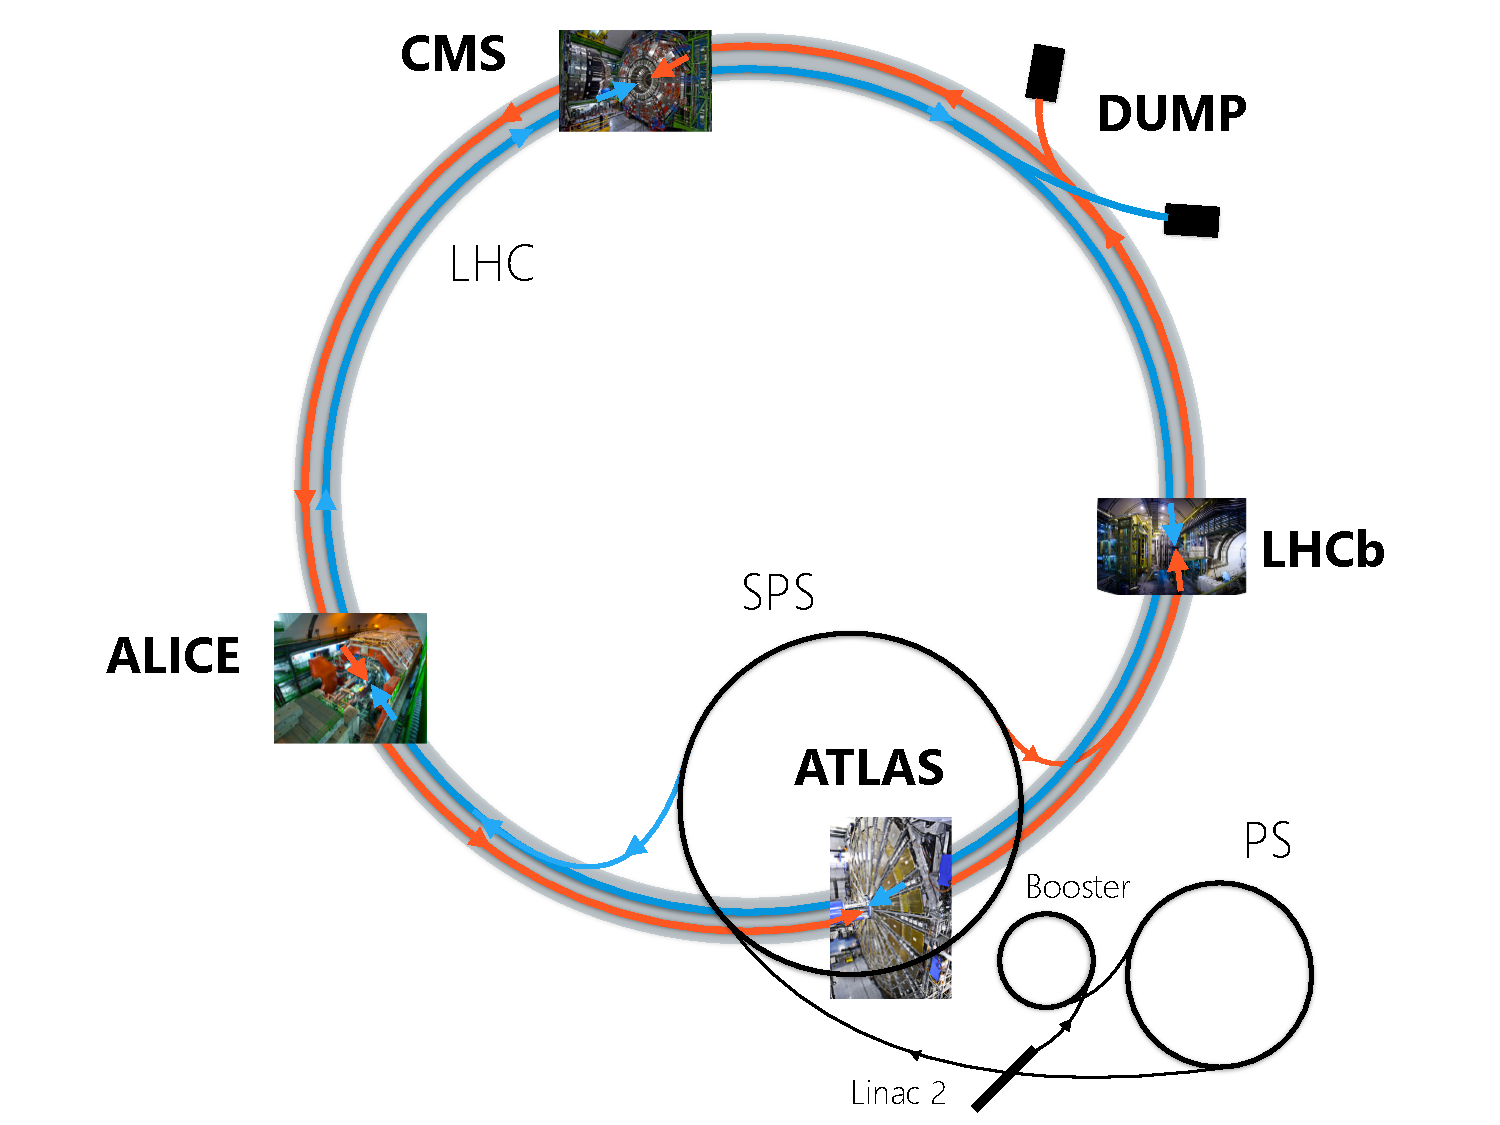
\includegraphics[width=\textwidth]{Figures/theory/Masterthesis_diagrams_SM/Masterthesis_diagrams_LHC.pdf}
    \caption[Schematic overview of the LHC accelerator complex.]{Schematic overview of the LHC accelerator complex condensed from Refs. \cite{cds_1,cds_2,cds_3,cds_openphoto_cms,cds_openphoto_atlas,cds_openphoto_alice,cds_openphoto_lhcb}. Before the protons enter the actual LHC ring,  
    they are pre-accelerated up to 450\,{GeV} in the accelerator chain beginning with the LINAC 2. 
    The particles increase their energy in the Booster and become further accelerated in the Proton Sychrotron (PS). 
    They reach an energy of 450\,{GeV} in the Super Proton Synchrotron (SPS). At the end of its lifetime the beam 
    is directed into a block of carbon, the \textit{beam dump}, to not damage the machine.}\label{CMS:LHC_overview}
\end{figure}
\section{The CMS Detector}

The 12.9\,{m} long superconducting solenoid with a field strength of 3.8\,{T} is the key feature of the \textit{Compact Muon Solenoid} (CMS). The detector
is built around the interaction point covering almost 4\textpi{} of solid angle and is designed to handle the high luminosities present at the LHC to measure and reconstruct
every particle produced in the 40 million bunch crossings every second. The volume within the magnet's internal diameter of 6\,{m} 
is large enough to contain the three layers of silicon pixel detector\footnote{From 2017 on, a new pixel detector is installed with a fourth layer.} very near to the interaction point, the silicon strip detector, the electromagnetic calorimeter (ECAL) 
and the hadronic calorimeter (HCAL). The muon system is embedded in the iron return yoke outside of the magnet and consists of three to four layers depending on the 
part of the detector \fref{CMS:Front_view}. 
 As in the following only a brief overview on the functionality of the detector components is given, the  reader is pointed to Refs.
\cite{CmsTdr1,Chatrchyan:1129810,} for a more detailed description. 

\begin{figure}[h]
    \centering
    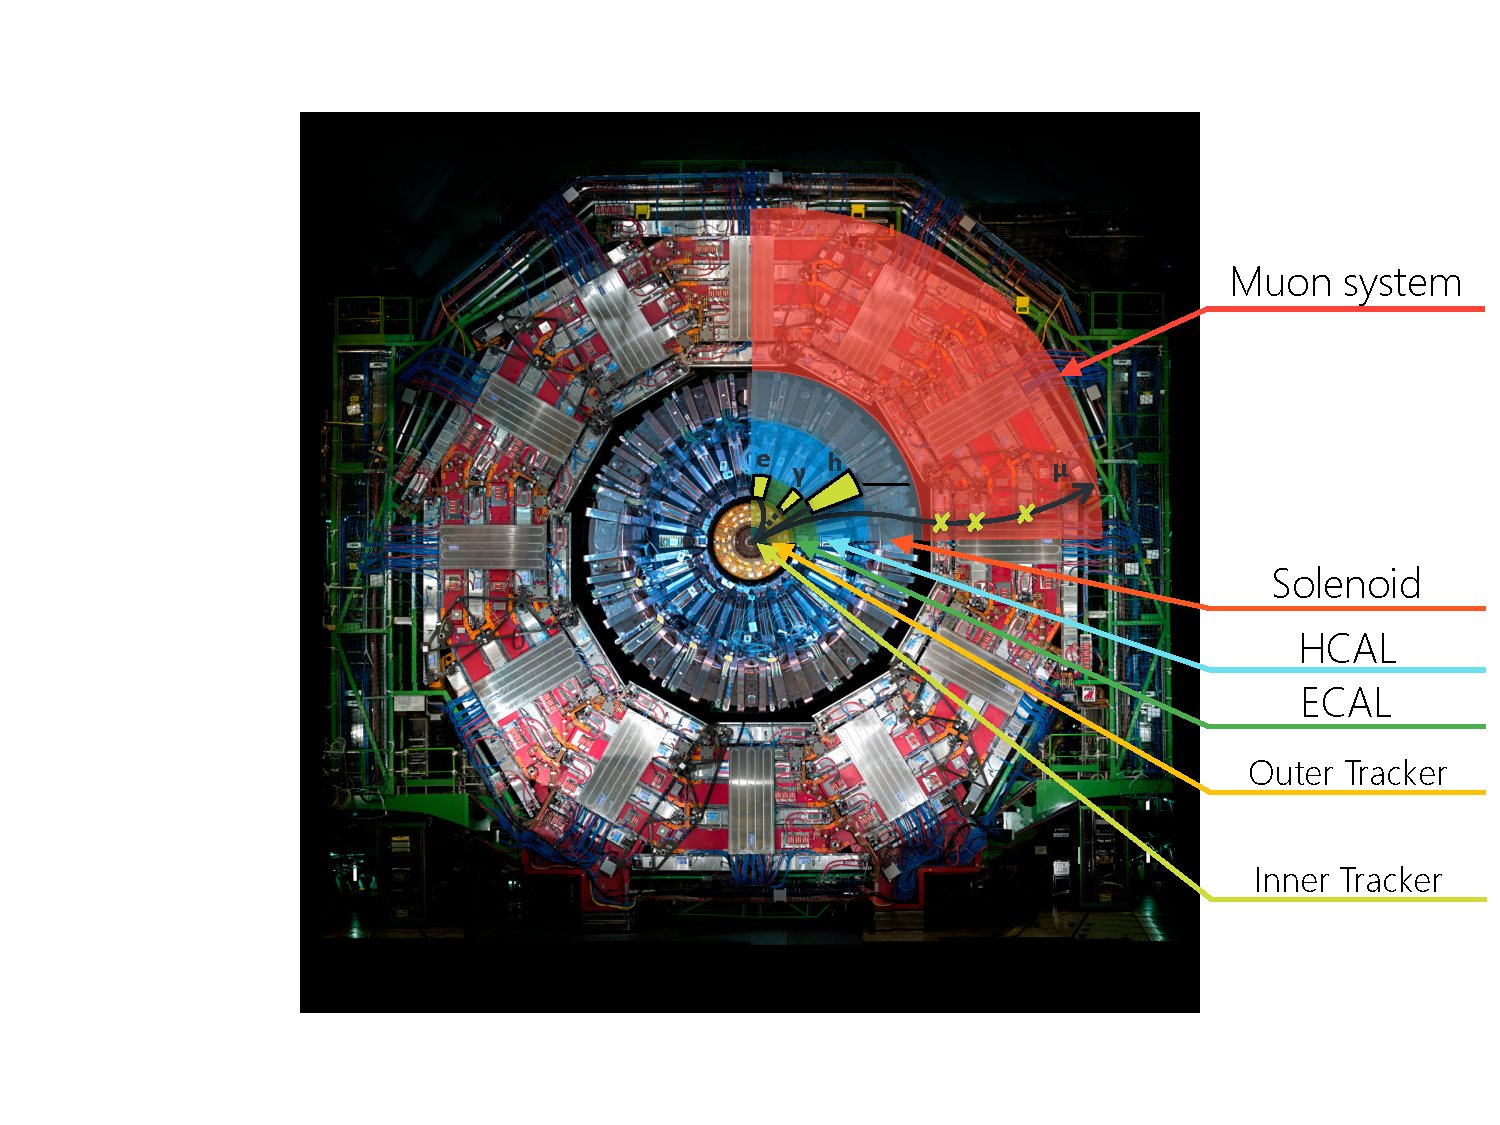
\includegraphics[width=\textwidth]{Figures/setup/CMS_front_view_modified}
    \caption[CMS Detector front view.]{Cross section of the CMS detector with highlighted subdetectors. Muons are the only known particles (except for neutrinos that cannot be detected directly with CMS) that traverse the whole detector. They leave signals in the tracker, the calorimeters and the muon system. Hadrons are detected with information 
    of the HCAL and leave signals in the tracker if they possess electric charge. The same holds for electrons that leave a record in the tracker and an energy deposit in the ECAL. Photons on the other hand 
    do not interact with the tracker but deposit their energy in the ECAL. Adapted from Ref. \cite{cds_openphoto_cms_frontview}.}\label{CMS:Front_view}
\end{figure}

\subsection{Detector subsystems}

\subsubsection{Tracker}

\begin{figure}[h]
    \centering
    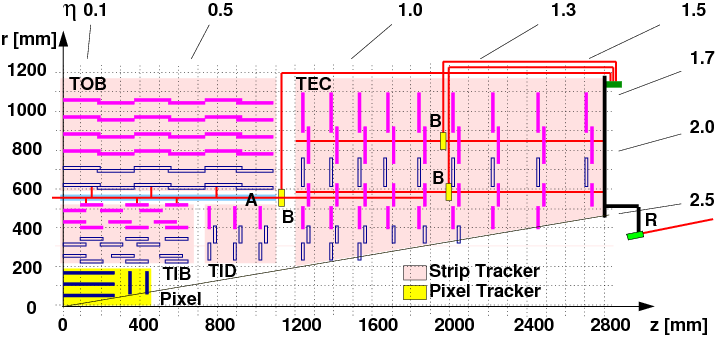
\includegraphics[width=.8\textwidth]{Figures/setup/tracker}
    \caption[CMS tracker layout.]{Layout of the cylindrical CMS tracker in the $\text{r-z}$-plane. The overall tracker covers pseudorapidities up to $\abs{\eta}=\text{2.5}$ and is made up of the pixel detector highlighted in yellow and the 
    strip detector in rose. The pixel detector is constructed such that every particle within $\abs{\eta}<\text{2.5}$ traverses at least three layers of pixel modules.
    Tracker inner and outer barrel (TIB and TOB) provide ten layers of tracking modules accompanied by three layers of inner disk modules (TID) and up to nine layers of endcap disks (TEC).
    A laser alignment system (LAS - in red) is used to monitor the exact position of each module in the detector to ensure highest accuracy during the track reconstruction. Taken from Ref. \cite{Chatrchyan:1211825}.}\label{CMS:tracker}
\end{figure}
The tracker is designed to measure the trajectories of charged particles. 
A silicon pixel detector with fine granularity is installed directly around the interaction point. The 
pixel detector is surrounded by the strip detector with a slightly broader granularity. 
The layout of the tracking system is depicted in \figreft{CMS:tracker}.
Charged particles ionize the semiconducting material when they traverse it. As a consequence electrons are elevated into the
conduction band, if an electric field is applied to deplete the sensor, and induce a small electrical current.
The high number of in total 66 million pixels and 9.6 million strips, that are each read out individually, leads to a channel occupancy which enables the tracking
system to confidently assign tracks by combining the signals of the charged particles produced during every bunch crossing. 
Tracks are the key ingredient for the identification of charged particles and reconstruction of the event vertex.

\subsubsection{Electromagnetic calorimeter}

% Add a picture of a lead-tungsten crystal.
The ECAL measures the energy of electrons, positrons and photons by total absorption. It covers a region up to $\abs{\eta}=\text{3.0}$ and consists of
61200 homogenous lead-tungsten (PbWO\textunderscript{4}) mono-crystals in the barrel and 7324 in the endcaps that produce scintillation light proportional to the energy of the stopped particle. The light
is collected and amplified by Avalanche Photodiodes (APDs) in the barrel region and Vacuum phototriodes (VPTs) in the endcaps. A preshower
device is installed in front of the endcap ECAL to detect $\pi^0$ decays. 

\subsubsection{Hadronic calorimeter}
The HCAL is a sampling calorimeter surrounding the ECAL that measures the energy of the hadronic activity. It is constructed to maximize the 
material within the coil of the magnet in terms of interaction lengths $\lambda$. Brass plates used as absorber are interspersed by plastic scintillator tiles 
which act as a compact active medium. Wavelength-shifting fibres transport the scintillating light to photosensors, which are connected to the read-out electronics located outside the 
barrel. To ensure hermiticity additional sets of scintillator tiles are installed outside the magnet coil to catch the tail of very high-energetic hadronic showers that are not stopped by the HCAL and the magnet. 
The HCAL in alignment with the ECAL covers pseudorapidities up to $\abs{\eta}=\text{3.0}$. In addition, a hadron forward calorimeter
made of steel and quartz fibres is installed in the region $\text{3.0}<\abs{\eta}<\text{5.0}$ to measure the forward hadronic activity.
Hadrons produce Cherenkov light in the quartz fibres that is detected by photomultipliers. 

\begin{figure}[h!]
    \centering
    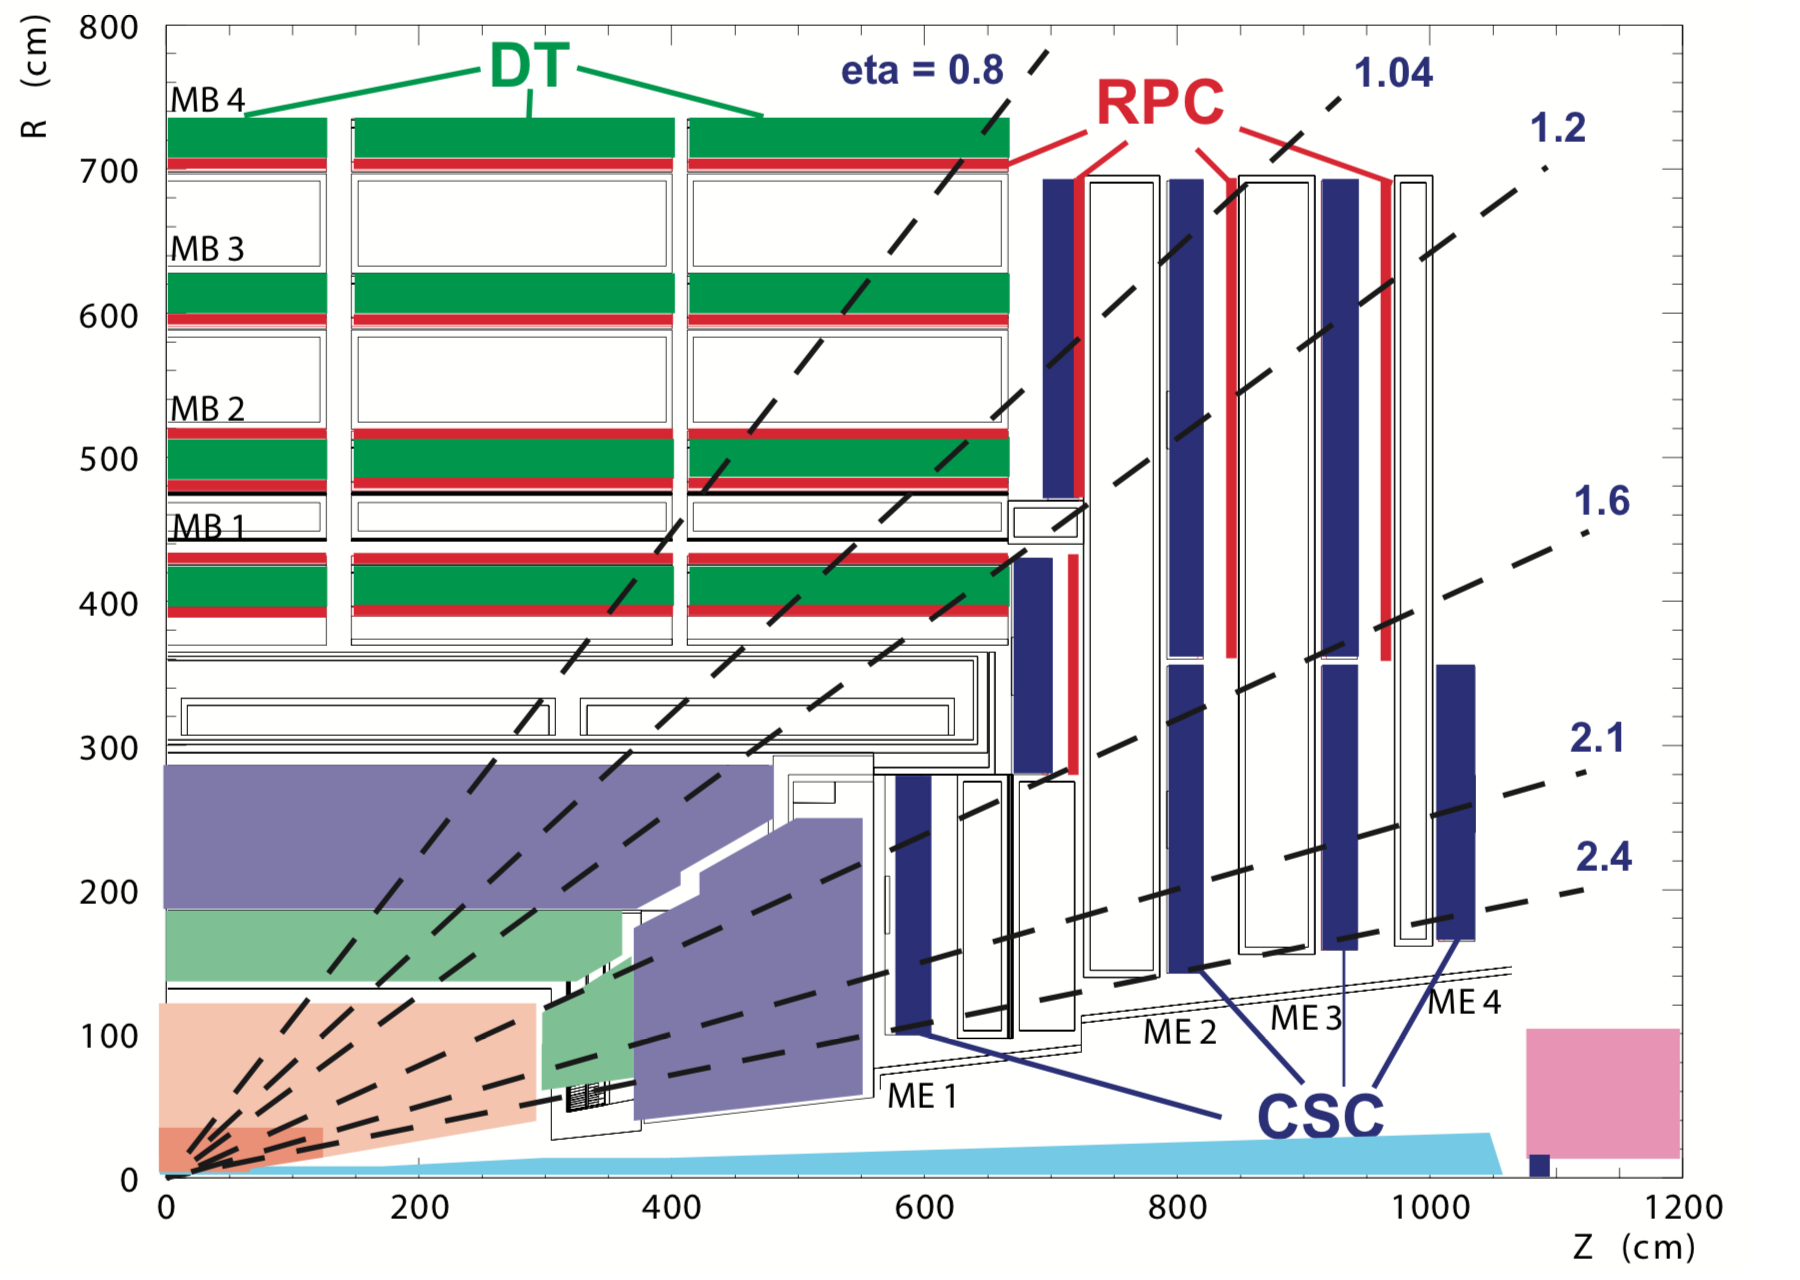
\includegraphics[width=.6\textwidth]{Figures/setup/muon_system}
    \caption[Muon chamber schematic view.]{Schematic view of a quarter of the muon system in the $\text{r-}\eta$ plane. Four layers of stacks of DTs (green) and RPCs (red) are installed around each wheel of the detector in the barrel region.
    RPC/CSC (red/blue) stacks are used to cover the region up to $\abs{\eta}=\text{1.6}$. Four layers of CSCs detect muons up to $\abs{\eta}=\text{2.4}$. Taken from \cite{CmsTdr1}.}\label{CMS:muon_system}
\end{figure}
 
\subsubsection{Muon chambers}

Muons are the only particles that pass through the whole inner detector and the solenoid.
The muon system uses three different types of gaseous detectors to identify muons. 
As indicated in \figreft{CMS:muon_system} the muon system is located  outside the solenoid.
The barrel covers pseudorapidities up to $\abs{\eta}<\text{1.2}$ and uses stacks of drift tubes (DT) and resistive plate chambers (RPC) to detect muons. The RPCs 
provide a very good time resolution as their response time is in the order of 1\,ns and make it subsequently possible to assign the correct bunch crossing.
In the endcaps the muon chambers operate in a higher magnetic field and must process higher muon rates. Therefore, six layers of cathode 
strip chambers (CSC) replace the DTs.\newpage{}
Overall, the muon system can measure muons with pseudorapidities up to $\abs{\eta}<\text{2.4}$.
Muons leave hits in both the tracker and the muon chambers and yield an exceptionally high track and primary vertex (PV) reconstruction precision for high energetic muons. 
The muon system is part of the trigger system to select interesting physics events.




\subsection{Trigger}
Due to technical limitations only about 100-1000 events out of the 40 million collisions taking place in CMS every second can
be written to tape and stored for high-level analyses. For this reason, the event rate must be reduced by a factor of $\text{10}^\text{5-6}$ using a sophisticated triggering system 
that is capable of extracting only the most relevant physics events within a couple of microseconds. CMS uses several stages of triggering. The electrical signals of all detector subsystems are stored in pipelined buffers while
the \textit{level-1} (L1) trigger, that is implemented in hardware, decides whether an event is kept or rejected. This decision is solely based on the primitive information of the calorimeters and the muon system. 
For this first step a computing time of 3.8\,{\textmu s} is allocated per event.
Events passing the L1 stage are feed into a processor farm where the high-level trigger (HLT) is applied that runs several menus of 
a lightweight reconstruction software. The HLT trigger is designed to reject events as early as possible. For this reason, the 
algorithms evaluate calorimeter and muon system data first and utilize the tracking system content and the full event information
only if the event was not disregarded in the first step. \newline{}
In 2016 the CMS Detector recorded proton-proton collision at a center-of-mass energy of $\sqrt{s}=\text{13\,TeV}$ with an integrated luminosity of $\text{L=35.9\,fb}^{-1}$. Recorded data is grouped into
so-called \textit{Runs} with similar quality assessment and detector performance. 2016 data from the Runs \textit{B-H} is used for this analysis.


\section{Particle Flow}

To perform a complex physics analysis, information provided by tracking, calorimeter and muon systems has to be
combined to reconstruct the actual particles produced in the collisions. At CMS, advanced reconstruction algorithms are 
applied to piece together particle signatures and find vertices. An iterative tracking reconstruction algorithm described in 
Ref. \cite{trackreco} uses hits in the tracker to reconstruct trajectories and vertices of charged particles. 
The energy of electrons, hadrons, and photons is inferred from energy deposit clusters in the ECAL and HCAL. Tracks and clusters are interpreted by the particle-flow (PF) algorithm \cite{1748-0221-12-10-P10003} that
links the reconstructed elements according to their spatial and kinematic compatability and tests which one of the five possible particle hypotheses describes the whole object. As a result, PF will give a list
of muons, electrons, photons, neutral and charged hadrons with the associated tracks and energy deposits. These particle candidates can further be
used to construct complexer objects, like \textit{jets}.
The reconstruction and selection criteria as used in this analysis are outlined in the following subsections. 
\clearpage
\subsection{Leptons}

\subsubsection{Muons}
Muons are required to be reconstructed by the PF algorithm. Thereby, muons are denoted  \textit{global} if a muon candidate based on muon chamber hits was matched to tracks in the inner tracker.
\textit{Tracker} muons are muons that were identified by assigning calorimeter and muon chamber entries to an already reconstructed inner track.
 In this analysis muons must pass the medium muon ID provided by the CMS collaboration \cite{muonID} with the requirements that the muon
\begin{ct_version_list}
    \item is reconstructed as a \textit{tracker} or \textit{global} muon, 
    \item has at least 49\% of valid tracker hits in data for Run B-F or 80\% valid hits for MC and data for Run G-H, and 
    \item is associated with the PV of the event by d\textunderscript{xy}<0.045\,{cm} and d\textunderscript{z}<0.2\,{cm}. Thereby, d\textunderscript{xy} and d\textunderscript{z} denote the transversal and longitudinal minimal distances between of the muon track and the PV.
\end{ct_version_list}
Furthermore, the muon must fulfill various quality criteria based on the performance of the fit.

\subsubsection{Electrons}
Electrons are reconstructed from energy deposits in the ECAL and tracks in the inner tracker.
They must pass the tight-working point of the multivariate-analysis (MVA) based electron ID corresponding to a 80\% electron selection efficiency.
To ensure that the electron is assigned to the PV, they must satisfy d\textunderscript{xy}<0.045\,{cm} and d\textunderscript{z}<0.2\,{cm}.

\subsubsection{Lepton isolation}

Lepton identification is made robust by isolating the lepton from other PF candidates around the lepton candidate within a cone of size $\text{\Delta R<0.4}$ ($\text{\Delta R<0.3}$) for muons (electrons) 
according to the formula
\begin{equation}
    I_\ell^\text{rel} = \frac{\sum p_\text{\,T} \li h^\pm \re + max\li \sum E_\text{T} \li h^0 \re + \sum E_\text{T} \li \gamma \re -\Delta \beta \sum E_\text{T} \li \text{PU} \re, 0 \re }{P^\ell_\text{T}}.
\end{equation}
The variable compares the transverse momentum of the candidate lepton $P^\ell_\text{T}$ with the sum of the transverse momenta of charged hadrons $p_\text{\,T} \li h^\pm \re$ and transverse energies of neutral hadrons and photons within the size of the cone.
Thereby, $\text{\Delta \beta = 0.5}$ is the estimate of the ratio of neutral to charged particles originating from additional proton collisions in the same event called \textit{pileup}\,(PU). 
Non-isolated leptons are likely to originate from heavy quark decays. In the analysis presented in the next chapter, leptons play an important role in identifying Higgs bosons. The isolation is a powerful observable to 
select leptons originating from the decay products of the Higgs boson. 
 
\subsection{Jets}
Jets originate from partons, generated in EW or QCD processes, for example. They undergo hadronization and create a collimated stream of particles that is seen as a cone shaped cluster of tracks and energy deposits in the detector.
As jets inherit the properties of the initial parton, it is crucial for the correct reconstruction of the jets to assign only those particles to the
jet that were really produced during hadronization. For this reason, dedicated sequential jet-finding algorithms have been developed that 
apply distinct angular distance criteria to combine particles in the detector to jets.
This analysis utilizes the \antikt{} algorithm \cite{antikt} with a cone size of $\text{R=0.4}$ to reconstruct jets. The algorithm clusters
individual particle flow candidates using a distance measure of the form 
\begin{equation}
    d_{ij} = \text{min}\li k_{ti}^{2p}, k_{tj}^{2p} \re \frac{\li \Delta y_{ij} + \Delta \phi_{ij} \re^2}{R^2},
\end{equation}
where $p=-1$ for the \antikt{} algorithm, $\Delta y_{ij}$ and $\Delta \phi_{ij}$ denote the rapidity and azimuthal differences, and the k\textunderscript{t} are the transverse momenta of the candidates.
By this, particles with large transverse momenta are clustered first, making the reconstructed jets particularly resistant against soft radiation, that is not originating from the hadronization process.
The jet properties are fully determined by the sum of all four-momentum vectors over all jet constituents. \\
To be considered in the analysis, jets are required to fulfill $\abs{\eta}<\text{4.7}$ and $p_\text{\,T}>\text{30\,{GeV}}$ and they must pass the jet ID \cite{CMS-AN-17-074}. Moreover, they must be separated by at least 
\begin{equation}
    \Delta R = \sqrt{\li \Delta\eta \re^2 + \li \Delta\phi \re^2} > \text{0.5}
\end{equation} 
from each of two reconstructed tau leptons. 
Jets originating from b-quarks usually emerge from a secondary vertex because the b-mesons have a relatively large lifetime and travel a non-neglibible distance in the detector before they decay.
Such jets are tagged by the Combined Secondary Vertex (CSV) algorithm and are considered \textit{b-tagged} if they pass the medium working point of the
b-tag ID provided by the CMS collaboration and have at least $\abs{\eta}<\text{2.4}$ and $p_\text{\,T}>20\unit{GeV}$.

\subsection{Tau leptons}
The hadron-plus-strips (HPS) algorithm \cite{hps1,CMS-DP-2017-006, CMS-DP-2017-002} is employed to reconstruct and identify hadronically decaying tau leptons, denoted by \tauh{}, by their decay mode \tabref{ES:tau_decaymodes}. Jets that were reconstructed by the \antikt{} algorithm in the previous step are taken as inputs for the algorithm.
From all electron and photon candidates with \pt{}>0.5\,GeV the one with the highest \pt{} seeds a $\pi^0$ candidate. Neutral pions decay almost immediately into a pair of photons.
Some of the photons convert in the tracker creating electron and positron tracks. Electrons and positrons may in addition radiate bremsstrahlung when crossing tracker material.
Thus, additional photon and electron candidates in a small $\phi-\eta$ window around the $\pi^0$ candidate are added. Such a cluster is called \textit{strip}.  
\tauh{} candidates are constructed from the charged hadrons and the neutral $\pi^0$s with $p_\text{\,T}>\text{2.5\,{GeV}}$.
Due to conservation of electric charge in the hadronic tau decay, only decay modes with an odd number of charged hadrons occur. 
Decays with one (three) charged hadron(s) in the final state are often called \textit{one-prong} (\textit{three-prong}) decays. The HPS algorithm combines decays with one charged hadron with 0, 1 or 2 $\pi^0$ candidates and
decay modes with three charged hadrons with no further $\pi^0$ candidate to \tauh{} candidates and calculates its four-momentum by summation of the four-momenta of the constituents.
To select a unique \tauh{} candidate the criteria given in table \ref{ES:tau_decaymodes} are applied. If a candidate can be assigned to more than one decay mode, the decay mode that maximizes the \pt{} of the \tauh{} candidate is selected.
Since \tauh's are reconstructed from jets, there is a high probability that a jets is misidentified as a tau lepton. Moreover,
the charged hadrons may be misidentified as electrons and muons and vice versa. For this reason, MVA-based discriminators are utilized to reject jets and electrons taking tau-lifetime variables and isolation 
of the \tauh{} candidate into account. Muons are vetoed using a cut-based discriminant. The discriminator against other jets are often referred to as the \textit{Tau ID}. \newline{}
Leptonically decaying taus are treated as if they were prompt leptons. Although tau leptons possess a relatively large lifetime and should be travelling some distance in the detector, it is rather challenging to identify leptons originating from tau decays. 
The determination of the impact parameter with respect to the PV is not very precise. Moreover, the large missing transverse energy (see section \ref{sec:MET}) coming from the two neutrinos in the leptonic decay is more or less balanced in the case that the decaying Higgs boson is not strongly boosted in the laboratory frame,
since the taus are produced more or less back-to-back in the lab frame, too. 
\begin{table}[!]
    \centering
    \caption[Tau lepton decay modes and branching fractions.]{Tau lepton decay modes and branching fractions ($\mathcal{B}$) with intermediate resonances. Charged hadrons are denoted by $h^\pm$ and neutral hadrons by $h^0$. The hadronic decay modes highlighted in
    light blue are reconstructed and used in this analysis. Adapted from Refs. \cite{nehrkorn} and \cite{Patrignani:2016xqp}.}\label{ES:tau_decaymodes}
    \begin{tabular}{ccccc}
        \toprule
        Decay mode  & Resonance    & \multicolumn{2}{c}{$\mathcal{B}$ / \% } & Selection \\ \hline
        Leptonic decays &           &   &   35.2 &  \\
        {\small $\tau^- \rightarrow e^-\bar{\nu_e}\nu_{\tau}$} &  &   {\small 17.8 } & &  \\
        {\small $\tau^- \rightarrow \mu^-\bar{\nu_{\mu}}\nu_{\tau}$} & &  {\small  17.4} & & \\ \midrule 
        Hadronic decays &           &   &   64.8  &  \\
        \rowcolor{ctcolormain!20}
        {\small $\tau^- \rightarrow h^- \nu_{\tau}$} &   & {\small 11.5}  & &  {\footnotesize No strips } \\
        \rowcolor{ctcolormain!20}
        {\small $\tau^- \rightarrow h^- \pi^0 \nu_{\tau}$ }& $\rho \li 770 \re$   &  {\small 25.9}  & & {\footnotesize One strip and $\text{0.3}<m_{\tau} <\text{1.3}\sqrt{􏰓p_\text{\,T}\text{/100\,GeV}}$}\\
        \rowcolor{ctcolormain!20}
        {\small $\tau^- \rightarrow h^- \pi^0 \pi^0 \nu_{\tau}$ }& $a_\text{1} \li 1260 \re$  &{\small 9.5 } & & {\footnotesize 2 strips and $\text{0.4}<m_{\tau} <\text{1.2}􏰓\sqrt{p_\text{\,T}\text{/100\,GeV}}$}\\
        \rowcolor{ctcolormain!20}
        {\small $\tau^- \rightarrow h^-h^-h^+   \nu_{\tau}$} & $a_\text{1}\li 1260\re$  & {\small 9.8 } & & {\footnotesize No strips and $\text{0.8}<m_{\tau} <\text{1.34\,{GeV}}$, $\text{\Delta z} <\text{0.4\,{cm}}$} \\
        {\small $\tau^- \rightarrow h^-h^-h^+ \pi^0 \nu_{\tau}$} &   & {\small 4.8 } & & \\
        {\small others} &   & {\small 3.3}  & \\ \bottomrule
    \end{tabular}%
\end{table}%
\subsection{Missing transverse energy}\label{sec:MET}
The missing transverse energy of the event is defined as the negative vectorial sum of the transverse momenta 
of all particles that are reconstructed by the PF algorithm in the event\,\cite{CMS_MET}
\begin{equation}
    \vec{E}_{\text{T}}^\text{miss} = -\sum_i \vec{p}_{\text{T},i}.
\end{equation}
